\documentclass[12pt,a4paper]{IEEEconf}

\usepackage{graphicx}
\usepackage{arabxetex}
\usepackage{fontspec}%  font  selecting  commands
\usepackage{xunicode}%  unicode  character  macros
\usepackage{xltxtra}  %  a  few  fixes  and  extras
%\usepackage{unicode-math}
\defaultfontfeatures{Scale=MatchLowercase}
\setmainfont[Mapping=tex-text]{Minion Pro}
\setsansfont[Mapping=tex-text]{Myriad Pro}
\setmonofont{Courier New}
\newfontfamily\arabicfont[Script=Arabic,Scale=1.5]{Adobe Arabic}

\author{Mohd Zamri Murah\\
\begin{affiliation}Pattern Recognition Group\\
Center for Artificial Intelligence Technology\\
Fakulti Teknologi Dan Sains Maklumat\\
Universiti Kebangsaan Malaysia\\
\end{affiliation}\\
\email{zamri@ftsm.ukm.my}}

\title{Design and Implementation of Jawi
keyboard layout: A Proposal}
\date{}

\begin{document}
\maketitle

\begin{abstract}
This paper presents a proposal for a Jawi keyboard layout based on Arabic(Saudi Arabia) keyboard layout. This layout allows the users to enter the six additional Jawi characters while maintaining the standard layout for the other Arabic characters. The main different between the two keyboards layout is that we change the positions for Arabic diacritical markings  into the positions to enter the six Jawi characters (\textarab{چ ,ڠ, ݢ ,ۏ ,ڤ, ڽ}). The layout would be familiar to those which Arabic background. The layout is not based on phonetic of the Jawi characters, for instance the arabic character alef \textarab{ا} is not map into the character 'a', thus may make it difficut for new users.
\end{abstract}

\section{Introduction}

There is currently no Malaysian standard for Jawi keyboard layout. Users who would like to write Jawi  face a difficult problem  because the current keyboard layout for Arabic doesn't support the additional six Jawi characters. Eventhough, there are various Jawi mapping available from various hardware manufactures for Jawi keyboard stickers and keyboards, each manufactures have their own Jawi layout mapping. This has make it difficult for Jawi users to write Jawi effectively.

In  this paper, we propose a standard layout for Jawi based on Arabic(Saudi Arabia) layout. This layout is choosen because;
\begin{enumerate}
\item it is the standard keyboard layout for the Arabic-writing world
\item it has mapping for all the Arabic characters used in Jawi
\item it is familiar to those with Arabic education background
\item it has minimal changes to the Arabic(Saudi Arabia) layout
\end{enumerate}
\section{Keyboard layout}

\subsection{The normal keyboard}

The propose Jawi keyboard layout for normal position is shown in figure~1. The position is similar to the Arabic(Saudi Arabia) keyboard layout.

\begin{center}
\begin{figure}[th] \label{fig:jawi1}
\caption{Position of Jawi characters in keyboard layout. It is the same with Arabic(Saudi Arabia) keyboard layout.}
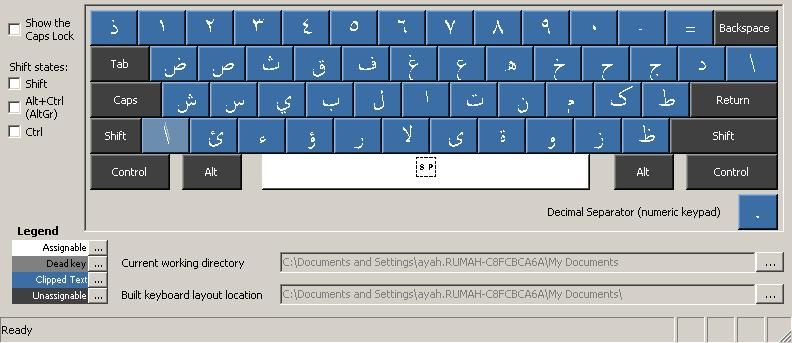
\includegraphics[width=\columnwidth]{Jawi.jpg}
\end{figure}
\end{center}

\subsection{The shift-position}

The propose Jawi keyboard layout for shift position is shown in figure~2. There are 7 changes in the Arabic(Saudi Arabia) keyboard layout positions; 6 diacritical markings are change into Jawi characters ( see on the upper left hand side of the keyboard ) and 1 diacritical marking for ZWNJ (Zero-Width None Joiner)( refer~\ref{subsec:zwnj}. All other positions remain unchanged. 

\begin{figure}[th] \label{fig:jawi2}
\caption{Position of Jawi characters in shift-position. There are six changes where 6 diacritical markings are changes into Jawi characters \textarab{چ ڠ ݢ ۏ ڤ ڽ} and 1 diacritical marking for ZWNJ.}
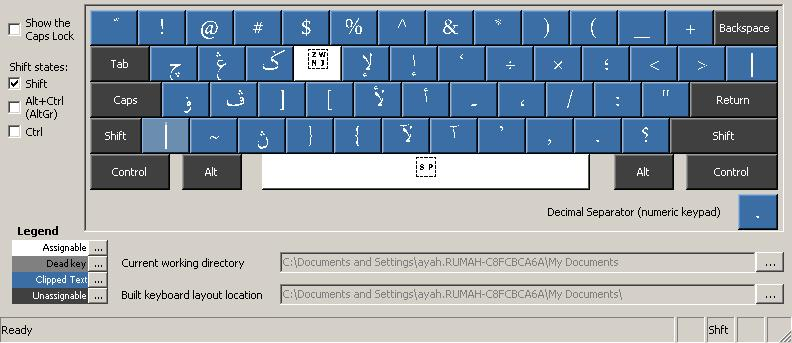
\includegraphics[width=\columnwidth]{JawiShft.jpg}
\end{figure}

\section{Discussion}

\subsection{Advantages}

The advantages of this jawi keyboard layout;
\begin{enumerate}
\item it is based on the standard Arabic keyboard layout. Since the standard Arabic keyboard layout is available on all computer platform, it is easier for users to install and use the Jawi keyboard layout. 
\item it has mapping for all the Arabic characters used in Jawi, thus reducing time to design a new layout for Jawi.
\item it is familiar to those with Arabic education background.
\item it make only 7 changes to the Arabic(Saudi Arabia) layout.
\end{enumerate}


\subsection{Disadvantages}

The disadvantages of this layout are;
\begin{enumerate}
\item not based on phonetic of the Jawi characters ( e.g the character 'a' for arabic character \textarab{ا}) or character 'b' for arabic character \textarab{ب} ). This probably will it difficult for new users to know the locations of each Jawi characters.
\item users may need to buy keyboard stickers or a new Arabic keyboard to use the mapping effectively. 
\end{enumerate}

\subsection{ZWNJ} \label{subsec:zwnj}

ZWNJ is an invinsible coding to separate Jawi words from joining. This is important in some words spelling. Example;
\begin{enumerate}
\item the word 'sains' is spell \textarab{ساءين‌س}, not \textarab{ساءينس}.
\item the word 'golf' is spell \textarab{ڬول‌ف}, not \textarab{ڬولف}
\item the word 'teks' is spell \textarab{تيک‌س}, not \textarab{تيکس}
\end{enumerate}

\subsection{tatweel}

Tatweel  (\verb|0640|) is an arabic character to stretch characters. 

For example;
\begin{enumerate}
\item without tatweel: \textarab{ساي سوکا جاوي}
\item with tatweel: \textarab{ســـــــــاي ســـــــوکــــــــا جـــــــــــاوي}
\end{enumerate}


\subsection{The mapping of \textarab{ݢ}}
There are two possible mapping of gaf ( or kaf with dot above) , \verb|06AC| (kaf with dot above ) and \verb|0762| ( keheh with dot above ) \cite{patterns1991unicode,davis2008moving}. Each however produce different ligature glyph based on initial, middle and final position of the characters. \cite{dan1988daftar}

The final (correct) output is application dependent, for instance \verb|notepad.exe| produce the correct final shape for both mapping. Some version on \verb|notepad.exe| on Window XP produces disjoint characters.

\begin{enumerate}
\item \textarab{\char"06AC} (\verb|06AC|) (kaf with dot above)

 \begin{enumerate}
 \item initial position: \textarab{ڬسا} 
 \item final position: \textarab{سڬ} ( the final ligature is wrong )
 \item middle position: \textarab{سڬي}
 \end{enumerate}

% shift ~ 06ac 
% shift-ctrl ~ 
% 12	E		0	062b	06ac	-1	0762	0762		// ARABIC LETTER THEH, ARABIC LETTER KAF WITH DOT ABOVE,
%  <none>, ARABIC LETTER KEHEH WITH DOT ABOVE, ARABIC LETTER KEHEH WITH DOT ABOVE
% 06AC ~ ARABIC LETTER KAF WITH DOT ABOVE
% shift-ctrl ~ 0762 ARABIC LETTER KEHEH WITH DOT ABOVE


\item \textarab{\char"0762} (\verb|0762|) ( keheh with dot above )
 
 \begin{enumerate}
 \item initial position: \textarab{ݢسا}
 \item final position: \textarab{سݢ}
 \item middle position: \textarab{سݢي}
 \end{enumerate}
\end{enumerate} 

The main problem is that not many fonts support \textarab{ڬ} on the \verb|0762| mapping.

\subsection{The mapping of  \textarab{ک} }

%27	OEM_1		0	06a9	003a	-1	0643	0643		// ARABIC LETTER KEHEH, COLON, <none>, 
% ARABIC LETTER KAF, ARABIC LETTER KAF

The letter \textarab{ک} can be map into \verb|06A9| (keheh) and \verb|0643|(kaf). Each produce a different final shape in a letter.

\begin{enumerate}
\item \textarab{\char"0643} \verb|0643| (kaf)
\begin{enumerate}
\item initial: \textarab{كلس}
\item middle: \textarab{سكي}
\item final: \textarab{سيك} (the final ligature is wrong)
\end{enumerate}

\item \textarab{\char"06A9} \verb|06A9| (keheh)
\begin{enumerate}
\item initial: \textarab{کيس}
\item middle: \textarab{سکي}
\item final: \textarab{سيک}
\end{enumerate}
\end{enumerate} 

\subsection{The proposal for \textarab{ݢ} and \textarab{ک}}

We propose the use of keheh(\verb|06A9|) and kekeh with dot(\verb|0762|) since both of them produce the correct final glyph in a word such as \textarab{سيک} and \textarab{سݢ}.

\subsection{The issue of hamza \textarab{ء}}

There are two hamza encoded; 
\begin{enumerate}
\item Arabic letter hamza (\texttt{U+0621}): {\textarab{\char"0621}}
\item Arabic letter high hamza (\texttt{U+0674}): {\textarab{\char"0674}}
\end{enumerate}

The position and the size of the two hamza are different.
Compare the use of the two hamza: \textarab{کبڠساءن}
and \textarab{کبڠسا\char"0674ن}.

In certain words, the correct position of \textarab{ء} is $3/4$ from the baseline. Compare the position of hamza using a standard font in the word \textarab{کبڠساءن} and the correct position of hamza in the same word \textarab{کبڠسا\raisebox{4pt}{ء}ن} . ( Notice the slightly shift upward position of hamza in the second word )

There are currently no fonts with hamza in $3/4$ position . However, a hack using subscript could be used, but the resulting line would be shift-up and would produce a rather imbalace document structure.

\section{update 26/10/2009}

\subsection{TC Multilingual keyboard layout}
The latest keyboard layout as agreed by TC Multilingual Group is different from this paper proposal. The keyboard layout is given in figure~3 and figure~4.

\begin{center}
\begin{figure}[th] \label{fig:jawi1}
\caption{Position of Jawi characters in keyboard layout. It is the same with Arabic(Saudi Arabia) keyboard layout.}
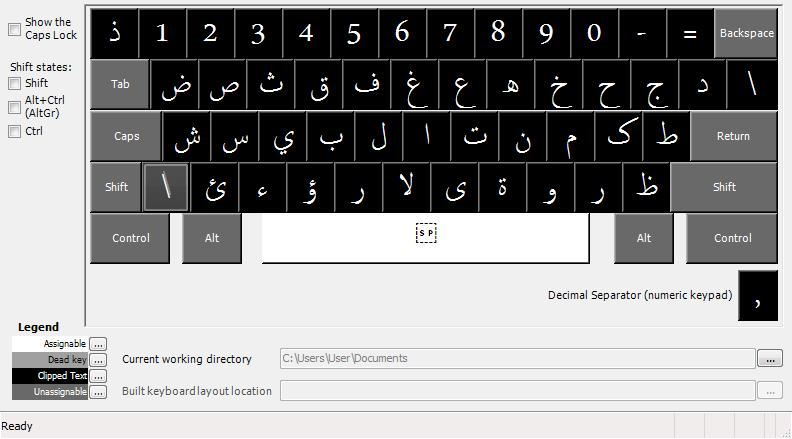
\includegraphics[width=\columnwidth]{arabjawi.jpg}
\end{figure}
\end{center}

\begin{center}
\begin{figure}[th] \label{fig:jawi1}
\caption{Position of Jawi characters in keyboard layout in shift position.}
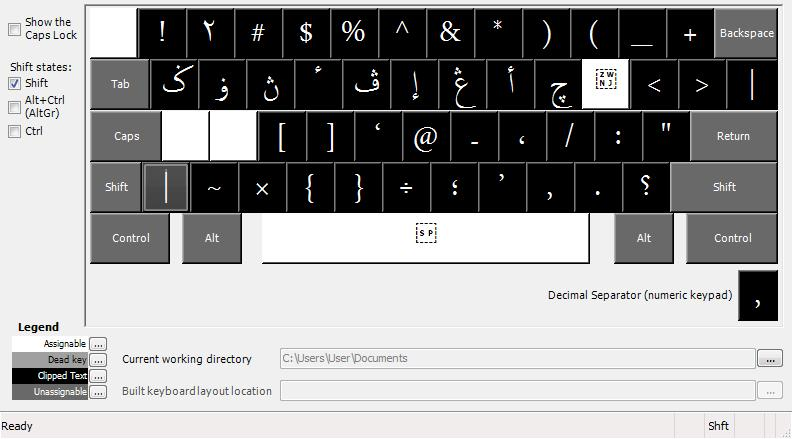
\includegraphics[width=\columnwidth]{arabjawiShft.jpg}
\end{figure}
\end{center}

\subsection{Amendments to be implemented}

The TC multilingual keyboard layout shift positions have these features;
\begin{enumerate}
\item a position for $3/4$ hamza in shift position. Currently, we do not have UNICODE encoding for $3/4$ hamza. A key is reserved for the future UNICODE for $3/4$ hamza.
\item the of high hamza  {\textarab{\char"0674}} as a temporary solution for the lack of $3/4$ in all fonts.
\end{enumerate}

\bibliography{jawi-keyboard-layout}
\bibliographystyle{plain}

\end{document}